% !TEX root = ../thesis-example.tex
%
%\chapter{Personalized Interaction via pointing gesture} \label{chapter:4}
\chapter{Personalized User Interface} \label{chapter:4}
Human centered computing aims at adapting computers to human minds and habits, and an important research direction in this area is the design of natural user interfaces and ergonomic human-computer interaction techniques.
Pointing gestures are fundamental to human behavior and are used consistently across cultures.
In section \ref{section:4-PAST}, we first propose a method to accurately recover the \textit{eye-rooted} pointing ray without tracking the eye gaze in an egocentric setting, enabling the user directly performing pointing gesture to interact with ambient media and objects without visual feedback. 
Then, section \ref{sec:4-IPCAI} introduces a novel personalized user interface, allowing the surgeon to personally perform touchless interaction with the various medical systems, and switch effortlessly among them, all of this without modifying the systems' software and hardware.

\section{Pointing gesture recovery in an egocentric setting}
\label{section:4-PAST}
Pointing gestures are fundamental to human behavior \citep{Matthews2012} and are used consistently across cultures  \citep{McNeill2000}. The gestures begin at an early developmental stage \citep{Carpendale2010} and let humans reference proximal objects as well as abstract concepts in the world. Today, pointing gestures are not only part of our gestural language but are inherently used for interaction \citep{Nanayakkara2013a}.
As shown in \figurename{\ref{fig:1-intro:problem}(a)}, there is a limited working zone when positioning a camera next to the monitor or on the ceiling to observe the user.
%Human centered computing aims at adapting computers to human minds and habits rather than the design of natural and ergonomic human-computer interaction techniques. 
As an alternative to the traditional setting of external sensors observing the user, an egocentric setting mounts a portable camera on the head or clothing of the user and perceives the interaction from an egocentric perspective \citep{Fathi2011,Li2015}. However, there is a significant angle between the ray starting from the camera and that from the eye when the user tries to point towards objects which are not reachable (see \figurename{\ref{fig:1-intro:problem}(c)} ).
%There has been significant recent interest in the egocentric approach to recognize the wearer's actions .
 
%Increasingly powerful wearable computers also advocate a tight integration between human and computer. 
%However, to perform a deep integration that offers timely cognitive and interactive support, the egocentric camera needs to better understand how humans interact with the world.
%A number of studies have demonstrated that pointing gestures perform quite effective selection in virtual environments \citep{Argelaguet2008} and interaction with very large, high resolution displays \citep{Vogel2005}.  

In this section we focus on how the pointing origin and geometry can be modeled in an egocentric setting, i.e. to understand the user-specific pointing gesture without external camera(s) or tracker(s) from the egocentric view. Regarding the ray's origin, pointing techniques can be classified into two groups: \textit{hand-rooted}, where the ray originates at the user's hand, and \textit{eye-rooted}, where the ray starts at the user's eyes. Whenever a \textit{hand-rooted} technique is used, the objects that are along the pointing ray might differ from those that the user focuses on \citep{Argelaguet2008}. The more interesting scenario is the latter. Thus, we focus on the \textit{eye-rooted} approach and demonstrate how to approximate and recover the pointing geometry within an egocentric setting.

The pointing gesture recovery in an egocentric setting would pave the way for performing real-time interaction with various digital objects and medias. 
With the similar viewpoint as the user, it allows the user to perform direct interaction with objects in the most natural way without relying in visual feedback. 
The pointing ray in the \textit{eye-rooted} technique is defined jointly by the user's eyes and fingertip positions.
\citet{Forsberg1996} specified that the choice of the origin point was an important consideration. This issue has been ignored in literature since: (i) the eye position is known in a virtual environment, and (ii) the user's dominant eye is customarily tracked using external cameras and trackers as the origin. Most often a visual feedback is also provided to improve the accuracy.

We propose a method to calculate a virtual eye center as the origin for the \textit{eye-rooted} pointing ray technique without tracking the eye gaze in an egocentric setting. The user specific pointing geometry can then be recovered for interaction with ambient media and objects without visual feedback. The pointing ray starts from the virtual eye center and goes through the fingertip to the desired target information. During the initial calibration, the user is asked to perform pointing gestures towards several targets displayed within the field of view. A user specific virtual eye center is then estimated based on the detected fingertip in the coordinate system of the wearable device. Then the \textit{eye-rooted} pointing ray is recovered when a user is performing a pointing gesture. We provide both a mathematical validation and a user study involving ten participants to assess the precision of our unique pointing gesture recovery.

\subsection{Methodology} \label{Methodology}
%\textbf{Symbol Description:}  $Tran_{d2c}$ transformation matrix of the color camera relative to the depth camera. 
\subsubsection{General Design} \label{sec:4:generalDesign}
In a general hardware design, the egocentric setup should include a wearable sensor, which is put on the user's head and that contains two sensors, $S_{f}$ and $S_{c}$. $S_f$ is used to detect the fingertip and calculate its 3D position. $S_c$ acquires the contextual information of the objects in front of the user. In general, $S_f$ should provide a near-range depth map as the 3D position of the fingertip has to be accurately calculated. 
{The contextual information is defined as the geometry and 3D position of the objects and medias perceived by the user.} $S_c$ can be a color camera, a depth sensor or a RGB-D sensor acquiring 3D position of given objects with known geometry or a valid depth map of the real world. 
As $S_{c}$ and $S_{f}$ are just different types of camera, the self-calibration of the wearable device can be performed using \citeauthor{Zhang2000}{\rq}s method \cite{Zhang2000}.

\subsubsection{Pointing At Several Targets (PAST) calibration} \label{sec:4:PAST}
Both human eyes perceive the visual information as a stereo camera and the images are processed by the brain to generate a 3D scene of the objects in the field of view. One always perceives a unified 3D scene no matter how we move our eyes. In other words, there could be a self-centered fixed origin point of the 3D scene in our brain, which we try to approximate as the virtual eye center. When performing pointing gestures, users always can directly position their fingertips somewhere between their eyes and the target generating a line of sight, which goes through the fingertip and the target. Using perspective-based pointing  \citep{Pierce1997},  the pointing geometry is modeled as a ray, which starts from the virtual eye center and goes through the fingertip towards the target, as shown in \figurename{ \ref{fig:past:calibration}}. It is important to emphasize that the virtual eye center is user specific and its location is affected by the fact that users may be left or right eye dominant (see \figurename{ \ref{fig:virtualEye}}).
%the user's specific pointing habit also impress the location (see \figurename{ \ref{fig:anotherHand}}). 
The PAST method accounts for this as its objective is to find the origin of the user specific pointing geometry. 
%Inspired by the Single-Point Active Alignment Method (SPAAM) for Optical See-Through head mounted display calibration for augmented reality \citep{Tuceryan2000},
A calibration is required to calculate the origin and the result is the position of the virtual eye center $E$. 
%Based on the pointing model, a set of pointing lines are collected to estimate the intersection to terminate the calibration. 
As shown in \figurename{ \ref{fig:past:calibration}}, the target $T_i$ is presented in front of the user, who is then asked to perform a pointing gesture towards it. The 3D positions of the fingertips $F_i$ and $T_i$ are collected through $S_f$ and $S_c$, respectively. The pointing ray $L_i$ ,which passes through $F_i$ and $T_i$, would also go through $E$. After enough pointing rays are collected, $E$ is defined as the best approximation of their intersection. After calibration, the user specific virtual eye center $E$ is estimated and the pointing rays can be recovered as $L_{i}$, going through $E$ and  $F_i$, when a pointing gesture is performed.
\begin{figure} 
	\centering
	\includegraphics[width= \linewidth]{figures/4-PAST/Figures/FIG2.pdf}
	\caption{The PAST Calibration. The user is asked to point at several targets $T_i$ using one finger. The pointing rays which pass through the fingertip $F_i$ and $T_i$ are collected. The intersection of these lines is $E$, the user specific virtual eye center.}
	\label{fig:past:calibration}
\end{figure}
\subsubsection{Target the user points at} \label{sec:4:findTarget}
%\subsubsection{Scenario with a wearable RGB-D sensor and a display} \label{sec:4:findTarget}
As defined in section \ref{sec:4:generalDesign}, {a mesh surface $M$ can be generated based on the contextual information which is observed via the sensor.}
After the PAST calibration, the user specific pointing geometry can be recovered as the pointing ray $L_{i}$. 
As shown in \figurename{ \ref{fig:pointToTarget}}, the intersection between $L_{i}$ and $M$ is $T_i$, the target which the user points at. No additional camera or marker is used to track the user's eye gaze or head and the user can directly interact with the media and objects in the real world using solely natural pointing gestures without any visual feedback. 
\begin{figure} 
	\centering
	\includegraphics[width= \linewidth]{figures/4-PAST/Figures/FIG3.pdf}
	\caption{The target the user points at. The intersection between the pointing ray $L_{i}$ and the $M$ is $T_i$, the 3D position of the target or information the user points at.}
	\label{fig:pointToTarget}
\end{figure}
%\subsubsection{Possible scenarios}
%\paragraph{A scenario with a wearable RGB-D sensor and a display}  {\label{sec:4:exampleScenario}} When the information is presented on a display, the depth sensor acts as $S_f$ and the color camera as $S_c$. 
%The 3D position of a fingertip can be calculated from a valid depth map when the pointing gesture is performed. It is very easy to detect a display and compute its plane function using image features. 
\subsection{Mathematical analysis of the PAST calibration}
The pointing gesture is fundamental to human behavior and is also quite personal \citep{Matthews2012}. If the images in the user's eyes were accessible, then $F_i$ , the fingertip detected in $S_f$, and $E$, the eye center calculated in the PAST calibration, would be perfect. 
In our proposed system, the user is asked to focus on the target and not on the fingertip. This allows the user to perform the pointing naturally.
In addition, the fingertip detection is based on a noisy depth image.
Thus, the fingertip used for pointing in the user's view is not always the same as the one detected by $S_f$. 
In this section, we first certify that there is a valid point $E$ for the collected pointing rays, even when the fingertip cannot be detected consistently. Then the accuracy of the recovered pointing ray is evaluated.

{As shown in \figurename{ \ref{fig:fingertipOffset}}, $F_i$  and $T_i$  are the fingertip and the target, which are detected by the wearable device. $E$ is the virtual eye center calculated through the PAST calibration procedure and $L_i$ is the pointing line estimated by the wearable device. If $\bar F_i$ and $\bar T_i$ are the fingertip and target in the user's own view, then a vector $V_{fi}$ can be defined to present the offset between $\bar F_i$ and $F_i$, $F_i = {\bar F_i} + V_{fi}$, when the pointing is performed.
During the calibration procedure, the user is asked to point towards a predefined target $T_i$, so ${\bar T_i} = T_i$ .
$\bar E$ is defined as the ideal virtual eye center and $\bar L_i$ is the ideal pointing line in the user's view. }
\begin{figure} 
	\centering
	\includegraphics[width= \linewidth]{figures/4-PAST/Figures/FIG4.pdf}
	\caption{ The pointing geometry during the calibration and recovery procedure. There is a vector $V_{fi}$  from $\bar F_i$ to $F_i$ when the pointing gesture is performed and a vector $V_{E}$, from the ideal virtual eye center ${\bar E}$ to $E$.}
	\label{fig:fingertipOffset}
\end{figure}
\subsubsection{Calibration} \label{sec:4:PASTCalibration}
Based on our model of the pointing geometry $\bar L_i$ is starting from $\bar E$ going through $\bar F_i$ and ending at the desired target $\bar T_i$. We use Eq.\ref{equ:pointOnLineUser} to  represent all the points along the pointing ray $\bar L_i$, and $\bar E$ is the intersection of all the pointing rays $\bar L_i$. 
\begin{equation}  \label{equ:pointOnLineUser}
P_{\bar L_i} = {\bar T_i} + \bar\lambda ({\bar F_i} - {\bar T_i}) ,\bar\lambda \in \mathbf{R} 
\end{equation}
This means that there is a $\bar\lambda = \bar \lambda_i$ making both Eq.\ref{equ:lambdaLineuser} and Eq.\ref{equ:intersectionOfLineUser} true for every  $\bar L_i$.
\begin{equation} \label{equ:lambdaLineuser}
\bar\lambda_i = \frac {D_{\bar E2 \bar T_i}}{D_{\bar E2 \bar T_i} -D_{\bar E2 \bar F_i}} 
\end{equation}
where $D_{\bar E2 \bar F_i}$ is the distance from $\bar E$ to ${{\bar F_i}}$ and $D_{\bar E2 \bar T_i}$ is the distance from ${\bar E}$ to ${\bar T_i}$. 
\begin{equation} \label{equ:intersectionOfLineUser}
{\bar E} = {\bar T_i} + \bar\lambda_i ({\bar F_i} - {\bar T_i}) 
\end{equation}
The pointing ray estimated by the wearable device is $L_i$, which goes through  ${T_i}$ and $F_i$. All the points along $L_i$ can be represented as:
\begin{equation} \label{equ:pointOnLineSensor}
P_{L_i} = {T_i} + \lambda(F_i - {T_i}) , \lambda \in \mathbf{R}  
\end{equation}
$F_i$ in Eq. \ref{equ:pointOnLineSensor} can be replaced by ${\bar F_i} + V_{fi}$ and ${T_i} = {\bar T_i}$ during calibration. Hence,
\begin{equation} \label{equ:pointOnlineSensor2}
P_{L_i} = {\bar T_i} + \lambda({\bar F_i} - {\bar T_i}) + \lambda V_{fi}, \lambda \in \mathbf{R}  
\end{equation}
There is a point $E_i$ on the line $P_{L_i}$, where $\lambda = \bar\lambda_i$ in Eq.\ref{equ:pointOnlineSensor2}.
\begin{equation} \label{equ:P_eye}
E_i = {\bar T_i} + \bar\lambda_i({\bar F_i} - {\bar T_i}) + \bar\lambda_i V_{fi}  
\end{equation}
After substituting Eq.\ref{equ:intersectionOfLineUser} into Eq.\ref{equ:P_eye}, there is always a point $E_i$ along every $L_i$ that can be represented as:
\begin{equation} \label{equ:P_eye2}
E_i = {\bar E} + \bar\lambda_i V_{fi}  
\end{equation}
\begin{figure} 
	\centering
	\includegraphics[width= \linewidth]{figures/4-PAST/Figures/FIG5.pdf}
	\caption{The curve of $\bar \lambda_i$. It decreases as $D_{\bar E2 \bar T_i}$ increases when $D_{\bar E2 \bar T_i}$ is fixed, and decreases as $D_{\bar E2 \bar T_i}$ decreases.}
	\label{fig:lambdai}
\end{figure}
%and the maximum length of  $V_{fi}$  is about the size of nail, 10 mm
%When PAST calibration is performed, we can fix the $D_{\bar E2 \bar T_i}$ and $\bar \lambda_i$ is only affected by $ D_{\bar E2 \bar F_i}$. 
As shown in \figurename{ \ref{fig:lambdai}}, $\bar \lambda_i$ in Eq.\ref{equ:lambdaLineuser} decreases slowly as $D_{\bar E2 \bar T_i}$ increases in three different example cases. $\bar\lambda_i$ can be rewritten as:
\begin{equation} \label{equ:lambdai}
\bar\lambda_i = \bar\lambda_c + \Delta \bar\lambda_i
\end{equation}
where $\bar\lambda_c = 1.15$ is the average and $\Delta \bar\lambda_i \in \left[-0.1,0.15\right] $, obtained from \figurename{ \ref{fig:lambdai}}. 
%the \textcolor{red}{Here, I want to express. $V_{fi}$ is a stable variable. And $\bar \lambda_i$  is also quite stable when during the calibration procedure as the distance to screen is fixed and the distance to fingertip is the user's habit. So $E_i$ is quite close and there is a valid $E$, the intersection of the lines $L_i$. Our calibration can get a valid result.}
$V_{fi}$ can be different every time as the depth map contains noise and the pose of the finger is different, hence it can also be represented as $V_{fc} + {\Delta V_{fi}}$, where $V_{fc}$ is a stable offset and ${\Delta V_{fi}}$ is a small random deviation. Thus,
\begin{equation} \label{equ:lambdavf}
\bar\lambda_i V_{fi} \approx  \bar\lambda_c V_{fc}  + {\Delta \bar\lambda_i} {\Delta V_{fc}} %+ \Delta \bar\lambda_i V_{fc} + \bar\lambda_c {\Delta V_{fi}}
\end{equation}
where $\bar\lambda_c {\Delta V_{fi}} + {\Delta \bar\lambda_i} {\Delta V_{fi}}$ is very small. As $\bar\lambda_c V_{fc}$ is consistent, $\Delta \bar\lambda_{i} V_{fc}$ is the main contribution of the variation for $\bar\lambda_i V_{fi}$. There is a candidate intersection point $E$, which is very close to all the lines $L_i$.
\begin{equation} \label{equ:P_eyeCalib}
E = {\bar E} + \bar\lambda_c V_{fc} 
\end{equation} 
The offset between $E$ and $\bar{E}$ is approximately $ \bar\lambda_c V_{fc}$. Even when there is about 2 cm offset between $F$ and $\bar{F}$, there exists a point $E$ and its distance to any line $L_m$ is not greater than 0.3 cm after substituting the numerical values in Eq.\ref{equ:P_eyeCalib}. Hence, there exists a valid approximation for the intersection of the pointing line $L_i$ making the PAST calibration feasible.
%Even when there is about 2 cm offset between $F$ and $\bar{F}$, there exist two points $E_m$ and $E_n$ along any two lines $L_m$ and $L_n$ respectively and the maximal distance between $E_m$ and $E_n$ is not greater than 0.3 cm. In other words there is a valid candidate point $E$, which is very close to of all the lines $L_i$. Hence, the PAST calibration is feasible and the offset between $E$ and $\bar{E}$ is approximately $ \bar\lambda_c V_{fc}$. 

\subsubsection{Pointing ray recovery} \label{sec:4:PASTrecovery}
As shown in \figurename{ \ref{fig:fingertipOffset}}, $E$ is the calibration result and there is an offset $V_{E} \approx \bar\lambda_c V_{fc}$, between $E$ and the ideal virtual eye center ${\bar E}$. 
When the user points towards a target after calibration, the position of the target calculated by the wearable device $T_i$, can be represented by $E$ and $F_i$ as:
\begin{equation} \label{equ:targetInSensor}
T_i = E+ \frac{D_{E2T_i}}{D_{E2F_i}}  \left( {F_i - E} \right)
\end{equation}
where $D_{E2F_i}$ is the distance from $E$ to ${{F_i}}$ and $D_{E2T_i}$ is the distance from ${E}$ to ${T_i}$. \\
$\bar T_i$ , the position of the ideal target in the user's view, can be expressed as:
\begin{equation} \label{equ:targetInEye}
\bar T_i \approx {\bar E} + \frac{D_{E2T_i}}{D_{E2F_i}}  \left( {{\bar F_i} - {\bar E}} \right)
\end{equation}
${\angle}_{E}$, the angle error between the user's pointing lines to $T_i$ and $\bar T_i$ can be calculated using Eq.\ref{equ:tanViewAngle} since $D_{E2T_i}$ is much larger than the offset between the targets $T_i$ and $\bar T_i$ . 
\begin{equation} \label{equ:tanViewAngle}
{\angle}_{E} \approx \tan^{-1} \left( {\frac{| {T_i - \bar T_i}| }{D_{E2T_i}} } \right)
\end{equation}
After substituting Eq.\ref{equ:P_eyeCalib}, Eq.\ref{equ:targetInSensor} and Eq.\ref{equ:targetInEye}, we get :
\begin{equation} \label{equ:tanViewAngle1}
{\angle}_{E} \approx \tan^{-1} \left( {{\frac{{\lambda_c{|V_{fc}|} }}{D_{E2T_i}} + \frac{{|\lambda_i V_{fi} - \lambda_c V_{fc}|} }{D_{E2F_i}}} } \right)
\end{equation}
As ${\angle}_{E}$ is very small, we get after substituting Eq.\ref{equ:lambdavf}:
\begin{equation} \label{equ:ViewAngleError}
{\angle}_{E} \approx \frac{ {\lambda_c{|V_{fc}|}} }{D_{E2T_i}} + \frac{ {|\Delta \bar \lambda_i V_{fc}|} }{D_{E2F_i}}
\end{equation}
\begin{figure} 
	\centering
	\includegraphics[width= \linewidth]{figures/4-PAST/Figures/FIG6.pdf}
	\caption{The curve of angle error. It decreases as $D_{E2T}$ increases and $V_{fc}$ decreases. $D_{E2F}$ does not really affect the accuracy of the pointing gesture.}
	\label{fig:evaluatinOfPointing}
\end{figure}
As shown in \figurename{ \ref{fig:evaluatinOfPointing}}, the angle error decreases as $V_{fc}$ decreases and $D_{E2T_i}$ increases. $D_{E2F_i}$ does not really affect the accuracy of the recovered pointing gesture. The accuracy of a recovered pointing line is below 0.9\degree in these four cases.

Based on the above feasibility analysis we can conclude that the PAST method can find a usable origin for the pointing ray which enables the wearable device to determine accurately where the user points to.
%The farther the distance of targets for calibration is, the smaller of the view angle error in any distance. Here we assume the $D_{E2F_i}$ is almost fixed as it is the habit of the user.
%The max view angle error can be calculated are 0.34\degree at 2 meter when $V_{fc} = 10mm$ and 0.67\degree when $V_{fc} = 20mm$. 
\subsection{Implementation}
%The current implementation in this paper is that $S_f$ is a depth camera and $S_c$ is a RGB camera.The main contribution of this paper is the calibration between wearable device and pointing system. So it does not matter which type of the $S_c$ is chosen when we evaluate the proposed calibration method. As shown in Section \ref{sec:4:findTarget}, the method to find the target is very similar with different contextual information.
In this section, we implemented a scenario with a wearable RGB-D sensor and two different displays. The 3D contextual information was acquired by tracking the display. During the PAST calibration process, the targets are shown on the display. The mesh, $M$, is then defined by the planar surface of the display. The display can be located at any angle and distance from the user.

\subsubsection{Hardware}
An Intel \textit{RealSense} 3D sensor  was selected as the wearable RGB-D device. It contains a 640x480 depth sensor (Valid Range = 0.2-1.2meters) and a 1920x1080 color camera. 
%The depth sensor $S_f$ is used to detect the fingertip  and the color camera $S_c$ to acquire 3D contextual information. 
The \textit{RealSense} 3D sensor was strapped on the user{\rq}s head using a bandana with an adjusted height and angle (see \figurename{ \ref{fig:hardWare}}). 
A 46$''$ TV display and a 24$''$ monitor presenting various information were positioned about the user as the contextual environment. 
The users could walk around and rotate their body or head freely while performing interactions with the display and monitor. 
%new finger with a raised finger TODO: retake a pircure of the hardware setup
\begin{figure}
	\centering
	\includegraphics[width = \linewidth]{figures/4-PAST/Figures/FIG7.pdf}
	\caption{The hardware setup. The side and front view of the wearable device. The \textit{RealSense} 3D sensor was strapped on the user{\rq}s head using a bandana.}
	\label{fig:hardWare}
\end{figure}
\subsubsection{Fingertip detection}
%The depth sensor and the color camera are packaged in one device and observe at the same direction. This resulted in not obtaining good contextual information and finger depth maps simultaneously. 
%todo needs a picture to show it clearly.
A real-time depth image of the hand or finger was generated via the near range depth sensor while the user performed pointing gestures. The depth sensor and the color camera were packaged in one device and were oriented in the same direction. When the color camera was adjusted to have a similar view as the user, there was no valid depth map of the full hand even when the user was asked to point upwards. Thus the fingertip detection technology developed by \citet{Betancourt2015a} was not employed. However, this limitation would be removed when a RGB-D sensor with the depth and color camera looking at different directions is developed commercially. In the meantime, with our current setup, the hand and finger blobs were directly extracted from the depth image using the \textit{Intel RealSense} SDK, and the contours and convex hull were calculated using the method provided by \citet{Suzuki1985}. The best peak was chosen as the detected fingertip position.

%\textcolor{red}{the following paragraph is not very clear}
%For each fingertip defect, there are 3 points: two peaks and the defect, as shown in \figurename{ \ref{fig:tips}} . We detect a fingertip in the first peak if the angle between the two peaks and the defect is lower than 90\degree and if the norm in pixel is higher than 15.
%\begin{figure} [h]
%	\centering
%	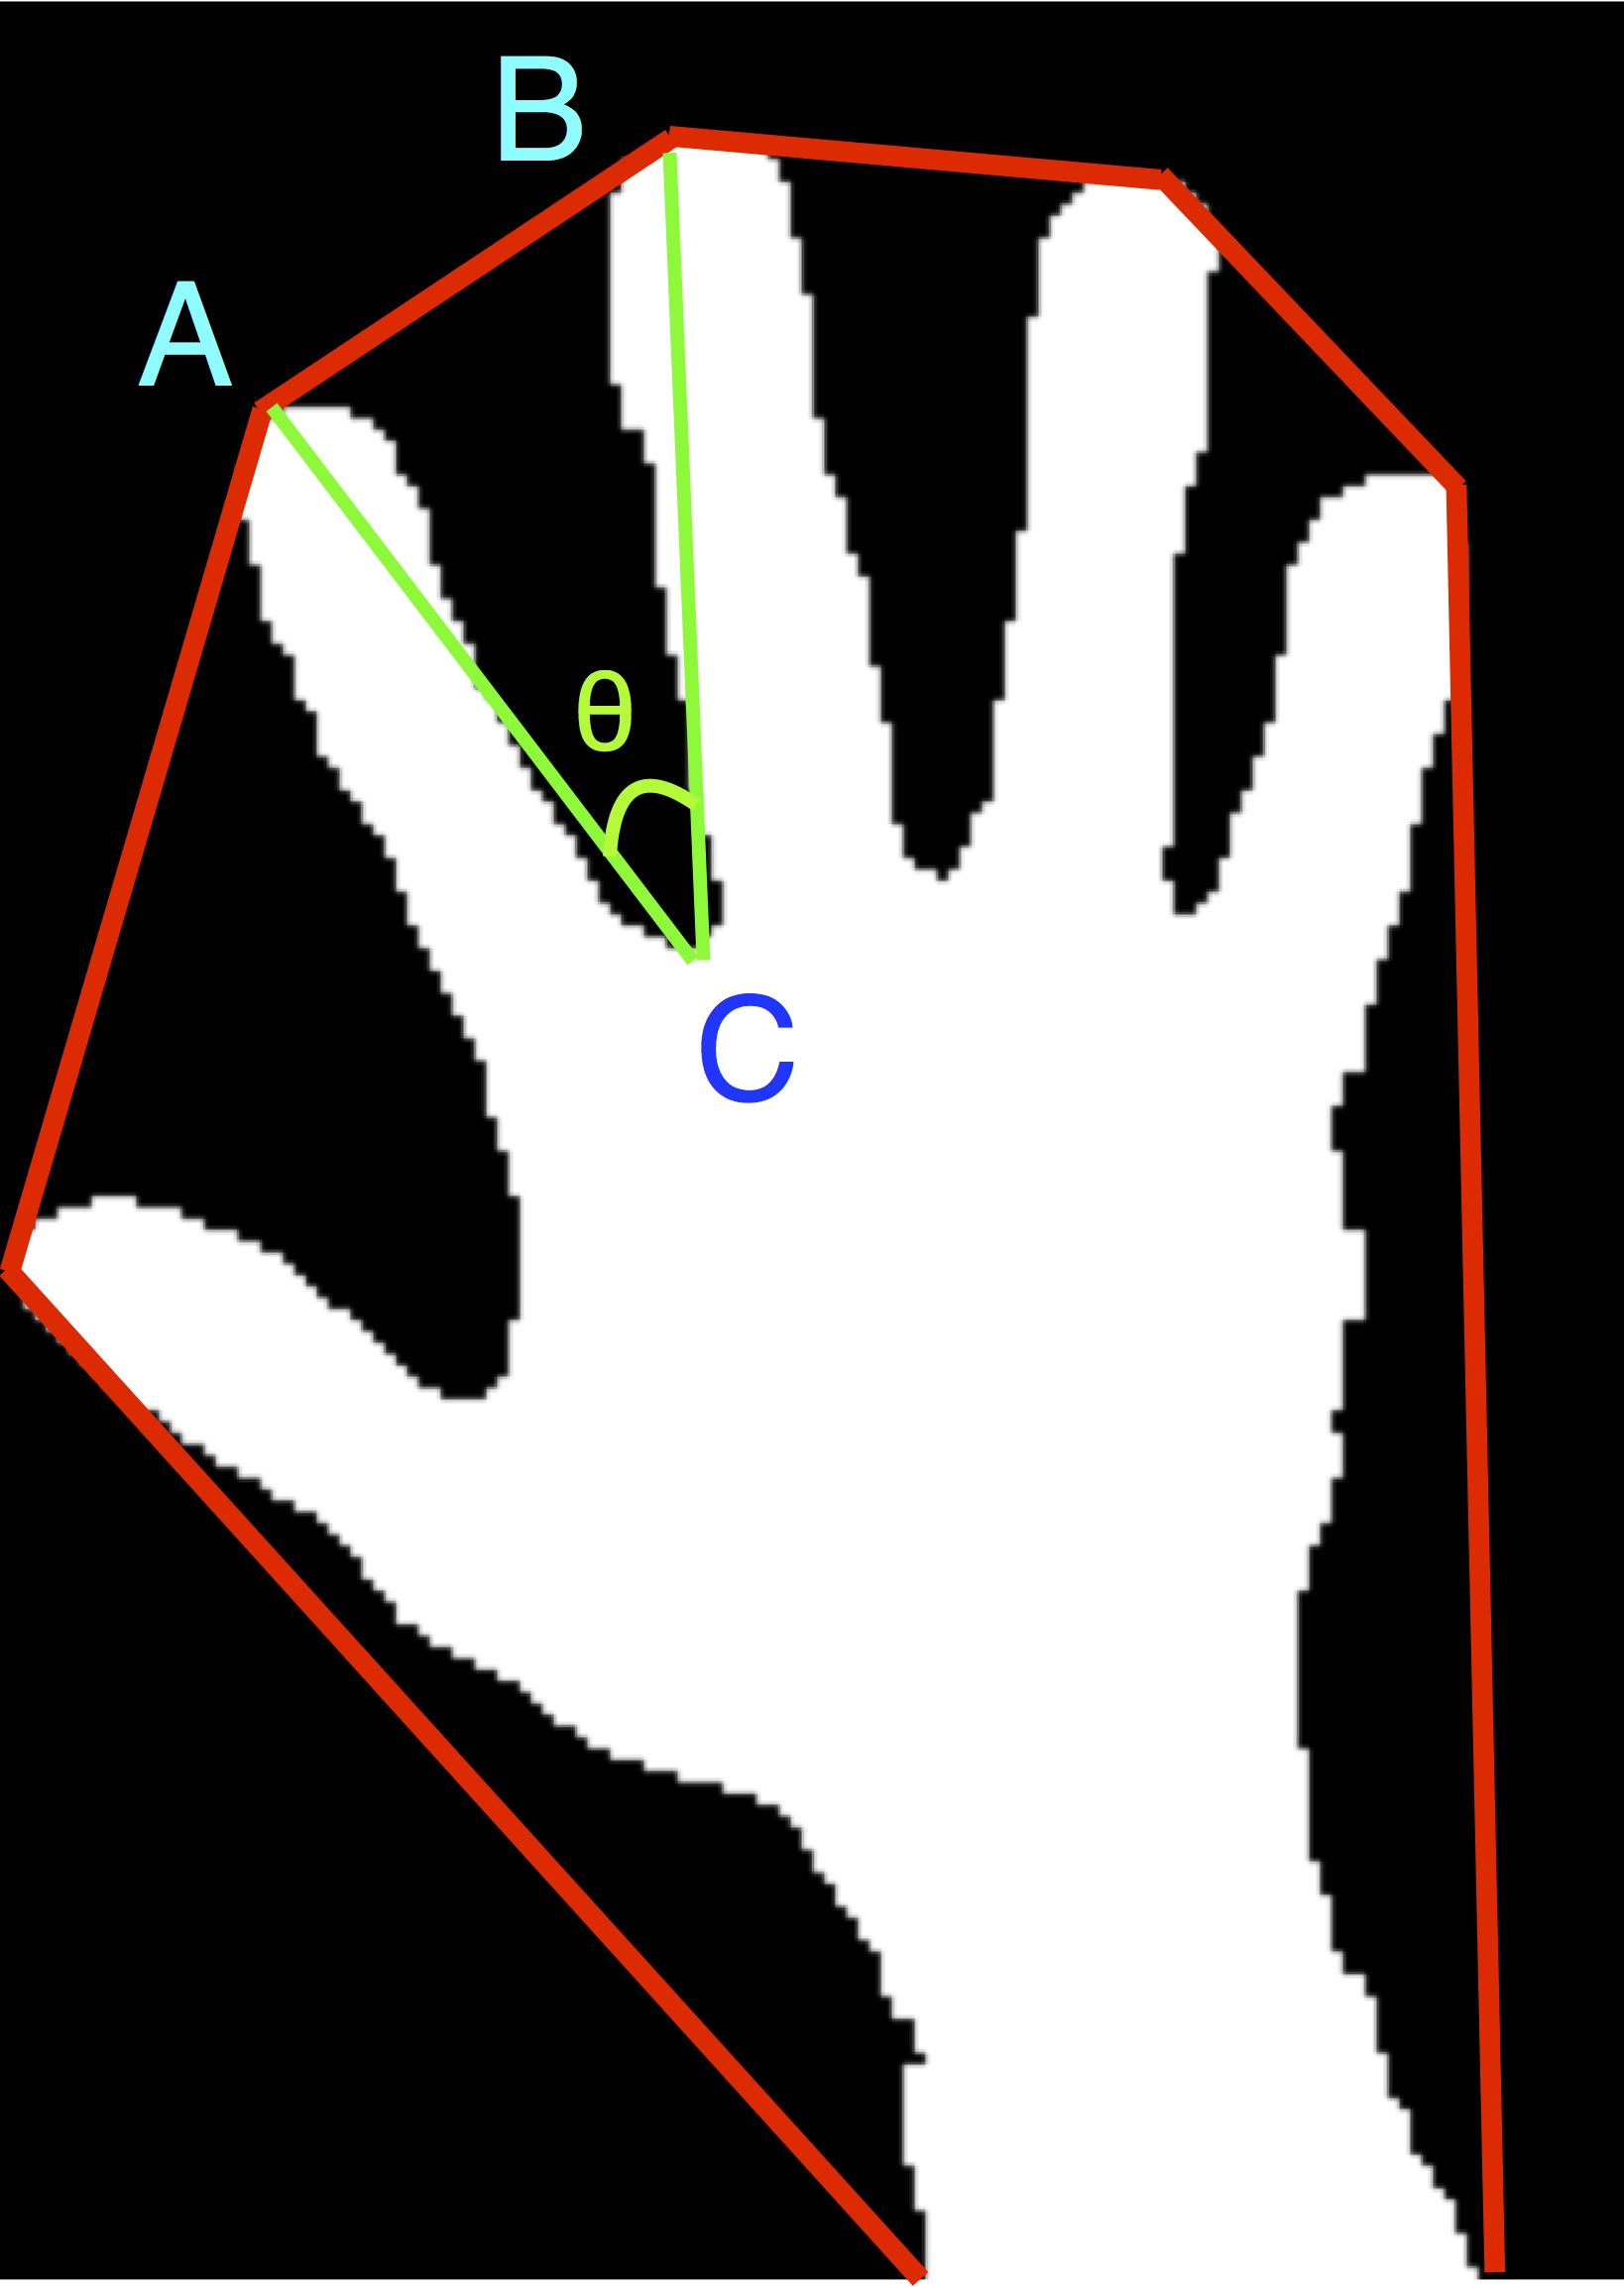
\includegraphics[width=1.5in]{figures/4-PAST/Figures/tips.jpg}
%	\caption {  We detect a fingertip in the first peak if the angle between the two peaks and the defect is lower than 90\degree and if the norm in pixel is higher than 15.}
%	\label{fig:tips}
%\end{figure}
\subsubsection{Contextual information} {\label{sec:4:markerDetection}}
To simplify the task of acquiring the contextual information, the \textit{ARTooKitPlus} \citep{Wagner2007a} markers were employed to track the TV display and monitor. There were two implementations: (i) some markers were directly displayed on the screen without interfering information (see \figurename{ \ref{fig:MarkerTracking}-left}). The markers were detected to calculate the planar function of the screen, and (ii) one physical printed marker was placed next to the display (see \figurename{ \ref{fig:MarkerTracking}-right}). A calibration was then performed to calculate the transformation matrix from the printed marker to the screen. The printed marker was then detected to calculate the information of the screen. 
As shown in \figurename{ \ref{fig:MarkerTracking}}, the screen was detected using the first implementation for the PAST calibration and evaluation, whereas the second implementation was employed during the \textit{DuckHunt} demo (see Section \ref{sec:4:PointingDemo}) and the medical application.
\begin{figure}
	\centering
	\includegraphics[width = \linewidth]{figures/4-PAST/Figures/FIG8.pdf}
	\caption{The contextual information. (1) Four \textit{ARTooKitPlus} markers shown on the display, (2) A target shown during the PAST calibration, (3) The \textit{DuckHunt} demo, (4) A printed \textit{ARTooKitPlus} marker. Left: During the PAST calibration, the screen was detected via the screen markers. Right: A printed marker was used during the \textit{DuckHunt} demo.}
	\label{fig:MarkerTracking}
\end{figure}
%todo: detection finger tip from two hand at the same time 
%	 how to describe the algorithm to simulate the mouse click 
%	 simple drawing demo using two hands at the same time
\subsubsection{\textit{DuckHunt} Demo} \label{sec:4:PointingDemo}
Inspired by the Nintendo game, a \textit{DuckHunt} demo\footnote{\url{https://youtu.be/Y4zO52oFDDg}} was developed using the pointing gesture to perform a dunk hunting task. Several flying ducks were shown on the screen and the user was asked to point to a duck to shoot it. 
After the completion of the PAST calibration, the user could directly perform a pointing gesture towards the screen to choose which duck to hunt without any visual feedback. The fire command was triggered when the user pushed the fingertip along the pointing line.

%\subsubsection{PictureView Demo} \label{sec:4:pictureviewDemo}
%In this section, a ``PictureView" demo was developed using the pointing gesture to perform interaction with screen. Several pictures were shown on the screen and the user was asked to select the picture and move it to a defined location, as shown in \figurename{ \ref{fig:MarkerTracking}}. After PAST calibration, the user could directly perform pointing gesture towards the screen to manipulate the picture as the wearable device could recover the pointing geometry and understand the spatial relationship between the pointing gesture and the pictures shown on the display. The selection command was recognized when the user pushed the fingertip along the pointing line. After selection, the picture was moved along the user's pointing gesture. When the picture was moved to the right area, the picture was dissociated with the pointing gesture and disappeared. Or the picture was also dissociated and reset to original position when moved to wrong area. See the supplementary video accompanying this paper.
\subsection{User study and results}
%todo: enroll 10 new user to perform the user study, with one eye case pointing, without calibration, pointing to ten targets and clock the user, (from different angle and distance, with or without feedback,  calibration is important: virtual eye as left eye, right eye, or the middle of the two eye. ). 
%todo: add an offset during the calibration procedure to remove the occlusion (compare the result with dominant eye pointing )
%questions: do we have to keep the first bared-hand cablibration 
To evaluate if a valid origin would be found by the PAST calibration and how accurate the recovered pointing ray was, we conducted a quantitative user study followed by qualitative evaluation to assess the proposed pointing technique in the egocentric setting. During the user study, several tasks were designed within different scenarios and the participants were asked to finish them and answer a questionnaire.

%Evaluation of the system: accuracy and precision for pointing and system usability to do the interaction with information shown on a screen or multi-screen.
\subsubsection{Scenario for experiments}
The TV display and the monitor were placed around the participant. There were three basic tasks for the user to perform during the user study:
%1) finish calibration using method A: the user chooses four targets in front of himself (for example the four corners of the TV display) and points at each target in different 
\begin{enumerate}[label=(\Alph*)]
	%Evaluation of Calibration method: time consuming and error
	\item \label{task:calib} \textit{Calibration:} a red target was shown at 9 different positions on the TV display and the user was asked to perform pointing gestures towards the target using their pointing finger.
	%The data is automatically collected when the user hold the finger still for one second.
	\item \label{task:pointEvaluation}\textit{Evaluation:} a blue target was shown at 9 different positions on the TV display or the monitor and the user was asked to perform pointing gestures towards the target using one finger. Data from 10 frames was collected and the average was calculated as the final result. 
	\item \label{task:PointWithFeedback}\textit{Evaluation with visual feedback:} a blue target was shown at 9 different positions on the TV display. The user performed pointing gestures using one finger towards the display and showcasing a green point as a visual feedback. The user was asked to match the green point and the blue target as close as possible. Data from 10 frames was collected and the average was used for accuracy analysis.
	
	%compare the time pointing to different targets in special order
	%\item \label{task:timeToMove} A target successively is shown in different places TV display and the user is ask to point at or move the cursor to target. 
	%\item \label{task:moveFiles} The user select one file shown at the TV display and move it to the monitor.
	%multi finger-interaction: one user and do the interaction with two hand at the same times
	%\item \label{task:drawing} To draw simple shape on the TV display: the user was ask to select one shape and then use one hand to decide the start position and another hand to change the scaling factor. 
\end{enumerate}
\subsubsection{Study description}
\paragraph{Participants} Ten people (6 Male and 4 Female, Age Range: 22-34) from different cultures were enrolled in the user study. Three of them grew up in Germany, three in China, two in Chile, one in France and one in India. Seven of them had a computer science degree. Nine were reported to be right-handed, while one was ambidextrous.

\paragraph{Study procedure} First, the participants put the wearable RGB-D device on their head and adjust the height and angle to make sure that the color camera has a full view of the TV display in front of them, while ensuring that the depth sensor had a valid depth map of their fingertip when performing the pointing gesture. Prior to beginning the user study, the participants were allowed to perform pointing gestures around the working environment and understood the volume in which their fingertip could be detected stably (this was limited by the field of view and pose of the depth camera). The user was asked to focus on the target of interest and not on their fingertip when performing a pointing gesture. After a simple training session, participants were asked to complete the following 10 steps for the evaluation. 
\begin{enumerate}[label=(\arabic*)]
	\item \label{step:stereoCalib} Perform task \ref{task:calib} three times from 2 meters away to complete the PAST calibration and evaluate if the calibration is stable. The first calibration result of the three is employed for all the remaining steps. 
	\item \label{step:pointWithFeedback} Perform task \ref{task:PointWithFeedback} on the TV display from 2 meters away, verify the calibration result, and calculate the accuracy the user can achieve with the visual feedback. 
	\item \label{step:pointingEvaluation} Perform task \ref{task:pointEvaluation} on the TV display from 2 meters away to evaluate the accuracy of the recovered pointing ray. 
	\item \label{step:diffentHand} Perform task \ref{task:pointEvaluation} on the TV display using the opposite hand from 2 meters away to evaluate if the calibration is independent of the hand.
	%one calibration: test with different hand and finger
	\item \label{step:distanceEvaluation} Perform task \ref{task:pointEvaluation} on the TV display from 1.5,3 and 4  meters away, to evaluate the accuracy of the recovered pointing ray at different distances.
	\item \label{step:differentScreenEvaluation}  Perform task \ref{task:pointEvaluation} on the monitor from 2 meters away to evaluate if the calibration is independent of the display.
	\item \label{step:calibDifferentDistance} Perform task \ref{task:calib} three times from 1.5, 3 and 4 meters away to evaluate if the calibration is independent of the target distance. 
	\item \label{step:calibOneEye} Perform task \ref{task:calib} with only the left or right eye open, from 2 meters away, to understand the relationship of the two eyes and the calculated virtual eye center. 
	\item \label{step:pictureview} Play with the \textit{DuckHunt} demo for 2 minutes using the first calibration result calculated in step \ref{step:stereoCalib}.
	\item \label{step:questionnaire} The interpupillary distance of the participant was measured with a ruler and the user completed a questionnaire to evaluate the pointing technique.
	
\end{enumerate}
%the detail step of the user study and the data to be collected
\subsubsection{Results} \label{sec:4:results}
%\aim{The calibration works well: we can get stable and reasonable result}
\paragraph{PAST Calibration} The real interpupillary distances of the ten participants were measured in step \ref{step:questionnaire}. They varied from 6.0 to 6.8cm (see \figurename{ \ref{fig:InterpupillaryDist}}). In step \ref{step:calibOneEye}, the calibration resulted in the positions of the left and right eye in the coordinate frame of the head-worn sensor system since the participants only used one eye. The interpupillary distances were also subsequently calculated from the distance of the two eyes. As shown in \figurename{ \ref{fig:InterpupillaryDist}}, the calculated distances were very close to the measured one using the ruler with an average difference of $0.10\pm0.05$cm. From this value, we conclude that the PAST method could accurately calculate the pointing ray origin based on the collected data. 
\begin{figure} 
	\centering
	\includegraphics[width=\linewidth]{figures/4-PAST/Figures/FIG9.pdf}
	\caption{Interpupillary distances. The calculated interpupillary distances of the 10 participants were very close to the ground-truth obtained using a ruler.}
	\label{fig:InterpupillaryDist}
\end{figure}
The average calibration results in step \ref{step:stereoCalib} were taken as the ground-truth to verify whether the PAST calibration was stable and independent of the scenario. 
For each participant, the offsets of the calibration results in step \ref{step:stereoCalib} and \ref{step:calibDifferentDistance} relative to the ground-truth are shown in \figurename{ \ref{fig:PAST}}.
The offset in the XY plane was less than 0.5 cm and that along the Z-axis was less than 1cm in most cases. The offset along Z-axis was larger than the XY plane since the PAST method estimated the intersection of the pointing rays which oriented towards the Z-axis. %, but it would not affect the pointing ray so much due to the same reason. 
The 3D distances from the virtual eye centers calculated at 1.5, 2, 3, and 4 meters away relative to the ground-truth were $0.60\pm0.35cm$, $0.56\pm0.41cm$,$0.90\pm0.73cm$, and $1.02\pm0.73cm$, respectively. 
%However the offset was still less than 1 cm in most cases.
The 3D distance calculated from 1.5 meters was greater than the one from 2 meters away, since $\bar\lambda_i$ increases as the $ D_{\bar E2 \bar F_i}$ decreases ( see section \ref{sec:4:PASTCalibration}).  
The offsets at 3 meters and 4 meters away were larger since the marker tracking accuracy decreased with increasing distance. The four plots in \figurename{ \ref{fig:PAST}} show that the PAST method could provide a stable calibration result for different users and the calibration is independent of the contextual environment. 
\begin{figure}
	\centering
	\includegraphics[width=\linewidth]{figures/4-PAST/Figures/FIG10.pdf}
	\caption{The calibration results in different scenarios. The results were compared to the reference one showing distribution of the offset along X,Y and Z-axis in the coordinate system of the wearable sensor. The XY plane was the one approximately parallel to the user's face. These four charts show the offset of the calibrations from different distances (a) 1.5 meters away (b) 2 meters away (c) 3 meters away (d) 4 meters away.}
	\label{fig:PAST}
\end{figure}
%\aim{The calibration result as origin point is good and the pointing ray is accurate in different case}

\paragraph{Accuracy of the pointing ray starting from $E$} 
The angle error of the recovered pointing ray, ${\angle}_{E}$, is calculated according to {Eq.\ref{equ:ViewAngleError}}. The precision is the difference of ${\angle}_{E}$ in 10 consecutive frames while the participant performs pointing gestures to the same target. ${\angle}_{E}$ turns out to be independent of the rotation of the participant, the size of the target and the spatial relationship with the target and the fingertip. To get a clear distribution of ${\angle}_{E}$, the vector from the $\bar T_i$ to $T_i$ is also calculated. As shown in \figurename{ \ref{fig:Accuracy2m}} and \figurename{ \ref{fig:Accuracy}}, for every point in the plots, the distance to the origin is defined as the angle value in degrees($\degree$), and the points are distributed according to the vector from $\bar T_i$ to $T_i$.
The first PAST calibration result in step \ref{step:stereoCalib} is employed to evaluate the pointing ray in different scenarios, with and without visual feedback, from different distances, and towards a different display.
The accuracy of the pointing ray with and without visual feedback is shown in \figurename{ \ref{fig:Accuracy2m}}. The accuracy with visual feedback is  $0.22\pm0.13\degree$ (see \figurename{ \ref{fig:Accuracy2m}(a)}).
The accuracy without any visual feedback from 2 meters away is $0.43\pm0.27\degree$ and ${\angle}_{E}$ is less than $1\degree$ as shown in \figurename{ \ref{fig:Accuracy2m}(b)}, which is consistent with the result presented in \figurename{ \ref{fig:evaluatinOfPointing}}. In addition, the precision of the pointing ray without visual feedback is  $0.10\pm0.07\degree$.
Comparing \figurename{ \ref{fig:Accuracy2m}(a)} and \figurename{ \ref{fig:Accuracy2m}(b)}, the pointing ray starting from the virtual eye center $E$ (the PAST calibration result), had the same level of accuracy as the case with visual feedback. Therefore, the pointing ray is accurately recovered in this scenario.
\begin{figure} 
	\centering
	\includegraphics[width=\linewidth]{figures/4-PAST/Figures/FIG11.pdf}
	\caption{After calibration, the participants performed pointing gestures towards some targets to evaluate if the pointing geometry could be correctly recovered. (a) with feedback at 2 meters away, and (b) without feedback at 2 meters away.}
	\label{fig:Accuracy2m}
\end{figure}

The pointing accuracies shown in \figurename{ \ref{fig:Accuracy}(a-d)} are $0.69\pm0.52\degree$ from 1.5 meters away, $0.63\pm0.44\degree$ from 3 meters away, $0.85\pm0.94\degree$ from 4 meters away, and $0.70\pm0.57\degree$ using a $24''$ monitor, respectively. 
As expected in \figurename{ \ref{fig:evaluatinOfPointing}},  ${\angle}_{E}$ increased at 1.5 meters away in \figurename{ \ref{fig:Accuracy}(a)}, compared to \figurename{ \ref{fig:Accuracy2m}(b)}. However, \figurename{ \ref{fig:Accuracy}(b) and \ref{fig:Accuracy}(c)} show that ${\angle}_{E}$ did not decrease when the pointing was performed from 3 and 4 meters away since the accuracy of the marker tracking declined. \figurename{ \ref{fig:Accuracy}(d)} demonstrates that the calibration was contextually independent and the pointing ray was still recovered when using the 24$''$ monitor. 
\begin{figure} 
	\centering
	\includegraphics[width=\linewidth]{figures/4-PAST/Figures/FIG12.pdf}
	\caption{The participants performed pointing gestures towards some targets in different scenarios to evaluate if the calibration was contextually independent. (a) perform pointing from 1.5 meters away (b) 3 meters away (c) 4 meters away and (d) perform pointing towards the 24$''$ monitor.}
	\label{fig:Accuracy}
\end{figure}

\figurename{ \ref{fig:Accuracy2m}} and \figurename{ \ref{fig:Accuracy}} show that ${\angle}_{E}$ is less than $1\degree$ in most cases in different scenarios. The overall pointing accuracy at 1.5, 2, 3, and 4 meters is $0.67\pm0.71\degree$. We conclude that using the PAST calibration result $E$, the virtual eye center can be set as the origin for the perspective-based pointing interaction and the pointing ray can be recovered accurately without any visual feedback.

%compare with uncalibration: not compare the system usability with relateive raycasting
%a good origin is very important to get an accurent pointing ray, camera view? 1 and 2 far away  eye as the origin 
\paragraph{Position of the virtual eye center} From step \ref{step:stereoCalib} and \ref{step:calibOneEye}, we obtained the positions of the virtual eye center and the two eyes in the coordinate system of the wearable device. When all interpupillary distances were upscaled to 7 cm, the spatial relationship of the left eye, right eye, and the virtual eye center could be drawn in a 2D plane (see \figurename{ \ref{fig:virtualEye}}). For four participants, the virtual eye center was very close to the left eye and these participants were determined as left-eye dominant using the method from  WikiHow\footnote{WikiHow:\url{http://www.wikihow.com/Determine-Your-Dominant-Eye}}.
\begin{figure} 
	\centering
	\includegraphics[width=\linewidth]{figures/4-PAST/Figures/FIG13.pdf}
	\caption{The spatial relationship of virtual eye center and the two eyes. The middle point of the two eyes was set as the original center and the calculated virtual eye center was shown in green.}
	\label{fig:virtualEye}
\end{figure}
The position of the virtual eye center was very user specific and influenced by the dominant eye. The potential positions of the origin for the pointing ray are the two eyes and the middle of them \citep{Forsberg1996}. These three points were ranked as close, middle, and far based on the distance to the virtual eye center $E$. The accuracy of the pointing rays starting at these three points is shown in \figurename{ \ref{fig:threeEyePositions}}. It is obvious that the point close to $E$ could be considered the best origin for the pointing ray. The PAST method can also be employed to estimate the origin when the eye positions are known.
\begin{figure} 
	\centering
	\includegraphics[width=\linewidth]{figures/4-PAST/Figures/FIG14.pdf}
	\caption{The accuracy of the pointing ray starting from the positions of the two eyes and the average of them. These three points were ranged as close, middle and far based on the distance to the virtual eye center $E$, calculated in the PAST calibration.}
	\label{fig:threeEyePositions}
\end{figure}
%However, we could not simply take the left eye, right eye, or middle point between the user's eyes as the virtual eye center to recover the pointing geometry. 
In step \ref{step:diffentHand}, the participants performed the pointing gesture using the opposite hand, different than the one used for calibration. In general, the results are good except for Participants 5 and 9 (see \figurename{ \ref{fig:anotherHand}}).  
Finally, the PAST calibration was dependent on the fingertip detected from the depth sensor and influenced by the user's specific pointing habit. The hand pose sometimes was quite different when the participant performed pointing with the opposite hand, thus the virtual eye center may be different for each hand.
\begin{figure} 
	\centering
	\includegraphics[width=\linewidth]{figures/4-PAST/Figures/FIG15.pdf}
	\caption{The accuracies of pointing with the opposite hand.}
	\label{fig:anotherHand}
\end{figure}
%However, we couldn't directly determine one participant was left-eye or right-eye dominant if the virtual eye-center calculated by PAST was very close to left or right eye respectively, since the PAST calibration was based on the user specific habit pointing gesture.
%questionnaire

\paragraph{System usability} To evaluate the proposed perspective-based pointing technique in an egocentric setting, a questionnaire was designed to obtain a qualitative evaluation. A Likert scale was used. The format of our 5-pt Likert was: (1) strongly disagree, (2) disagree, (3) neither agree nor disagree, (4) agree, (5) strongly agree. 
\begin{table}
	\caption{The Likert scale results of the questionnaire}
	\label{tb:4-pAST:questionnaire}
	\scriptsize
	\begin{center}
		\begin{tabular}{p{7.5cm}|p{1.2cm}}
			Questions & Scale \\
			\hline
			\textit{Q1:} I think that I would like to use this system &  $4.0\pm0.8$ \\
			\textit{Q2:} I found the system unnecessarily complex & $4.7\pm0.5$ \\
			\textit{Q3:} I thought the system was easy to use & $4.2\pm0.9$ \\
			\textit{Q4:} I don't think that I would need the support of a technical person to be able to use this system & $4.1\pm1.0$\\
			\textit{Q5:} I think the system is consistent & $4.3\pm0.6$ \\
			\textit{Q6:} I would imagine that most people would learn to use this system very quickly & $4.4\pm0.5$ \\
			\textit{Q7:} I felt very confident using the system & $4.3\pm0.6$ \\
			\textit{Q8:} I didn't need to learn a lot of things before I could get going with this system & $4.5\pm0.5$
		\end{tabular}
	\end{center}
\end{table}
As shown in \tablename{ \ref{tb:4-pAST:questionnaire}}, all questions attained positive scores above 4.0. Q1 had the lowest score as some participants felt a little tired while continuously lifting their arm to perform pointing gestures. In the ``DunkHunt'' demo, the fire command was recognized when the user moved their fingers along the pointing line, which was a little different from a natural click hand gesture. Therefore, the participants required some time to get used to it. In general the participants liked the pointing interaction with an egocentric setup and could learn it easily and quickly.

\subsection{Conclusion}
This section presented the Pointing At Several Targets (PAST) method to calculate an origin for the \textit{eye-rooted} pointing ray and recover the user specific pointing geometry in an egocentric setting without external cameras and trackers. 

This work is different from the state-of-art techniques for hand gesture recognition and gesture based interaction. Its main difference lies in calculating the ray origin for the user's specific habit, recovering the pointing geometry accurately, and enabling direct interaction with real and virtual digital elements of interest within the user's environment without any visual feedback.
%One problem that arises from allowing any wearable device always to understand the spatial relationship between the user's specific pointing gesture and the ambient information within the mixed reality world, is to how to model and calibrate the user specific pointing gesture. 

Mathematical analysis and experimental results demonstrate that the PAST calibration can estimate the origin point stably and recover the user specific pointing ray accurately. The calibration method is contextually independent and in most cases the pointing line is recovered with an accuracy of less than $1\degree$. The overall pointing accuracy at 1.5, 2, 3, and 4 meters is $0.67\pm0.71\degree$. 
The PAST solution would enable a whole series of applications with an egocentric setting in which the user can directly acquire or interact with different media and objects in real-time. 
%It paves the path towards a seamless of integration between human and computer sciences: the user can
It will allow users to naturally perform multi-control interaction with virtual or real elements placed within their environment. 

In future work, one could improve the hand gestures command combined with the pointing gesture enabling multi-modal interaction. Moreover, this work offers the possibility of developing an intuitive method for selecting desired objects in a real scene thanks to the recovered pointing gestures.